\section{Hands-on examples for parallel programming (2)}\label{sec:hands_on_cuda_2}

\subsection{PyCUDA Module and Numba}
As you might have suspected from the last sections, the world of GPUs is vast and complex, and C is not the easiest and most readable language to use for your everyday coding. Understanding CUDA, its standards and its mechanisms is mandatory, but fortunately, fellow Python users, there are some ways to make our lives a little easier. 

PyCUDA is a powerful module that lets you access NVIDIA's CUDA parallel computation API directly from Python. This means all standard CUDA features can be easily accessed through it. PyCUDA supports Just-In-Time (JIT) compilation of CUDA kernels written in C, while maintaining a very small overhead with respect to a pure C implementation for the GPU part.  Furthermore, it provides several additional quality-of-life features, such as translating native CUDA exceptions into standard Python exceptions. One of the main virtues of PyCUDA is that it allows us to use the \texttt{GPUArray} class to handle memory transfers smoothly. We will dive deeper into all of this in the following examples.

Alongside PyCUDA, we will also use Numba to compile universal functions (ufuncs) directly on the GPU.

Here are some useful references on these two modules:
\begin{itemize}
    \item[-] \url{https://pypi.org/project/pycuda/}
    \item[-] \url{https://documen.tician.de/pycuda/}
    \item[-] \url{http://numba.pydata.org/numba-doc/latest/cuda/index.html}
\end{itemize}

\textbf{Google Colab}, also known as \textit{Colaboratory}, is a free \textit{Jupyter} notebook environment running on the Google Cloud. It provides an accessible environment to write text and run Python 3 (and many other) code directly from your browser, with the notebooks being automatically stored in your Google Drive. One of its main advantages is the ability to run your code on cloud computers housing dedicated GPUs. Thanks to the underlying IPython library, it is also possible to execute shell commands---including compilers---directly on the cloud filesystem, as well as install and add new modules to your development environment. If you don't have a GPU to work with, you can start working on Colab (\url{http://colab.research.google.com}) to run your GPU-based programs.

For this section, we are going to use a Jupyter Notebook which you can find at the following link: \url{https://colab.research.google.com/drive/1C3bY-DKcyOp067Nti08JZ8cfnfz9YmCK?usp=sharing}. With respect to the corresponding notebook that you will surely find on the E-Learning page of the course, here some comments and notes have been added to make it more readable and clear. Try to run it on Colab or on your local PC.

Since I have to start a new page in order to input the Notebook in my LaTeX file, here is a photo of Dustin Brown executing a backhand volley against Rafael Nadal during the 2015 Wimbledon tournament. Brown went on to defeat Nadal in 4 sets with a flashy, fearless and dominant performance, with probably the best opening game in the history of tennis.

\begin{center}
    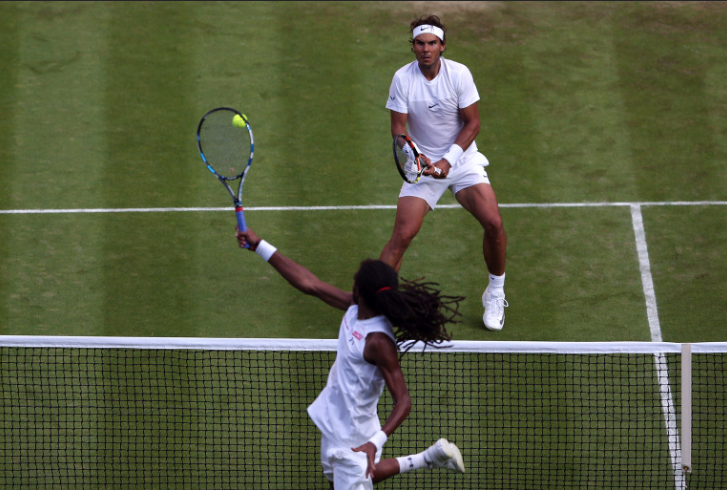
\includegraphics[width=0.3\textwidth]{figuresP/dustin_brown.png}
\end{center}

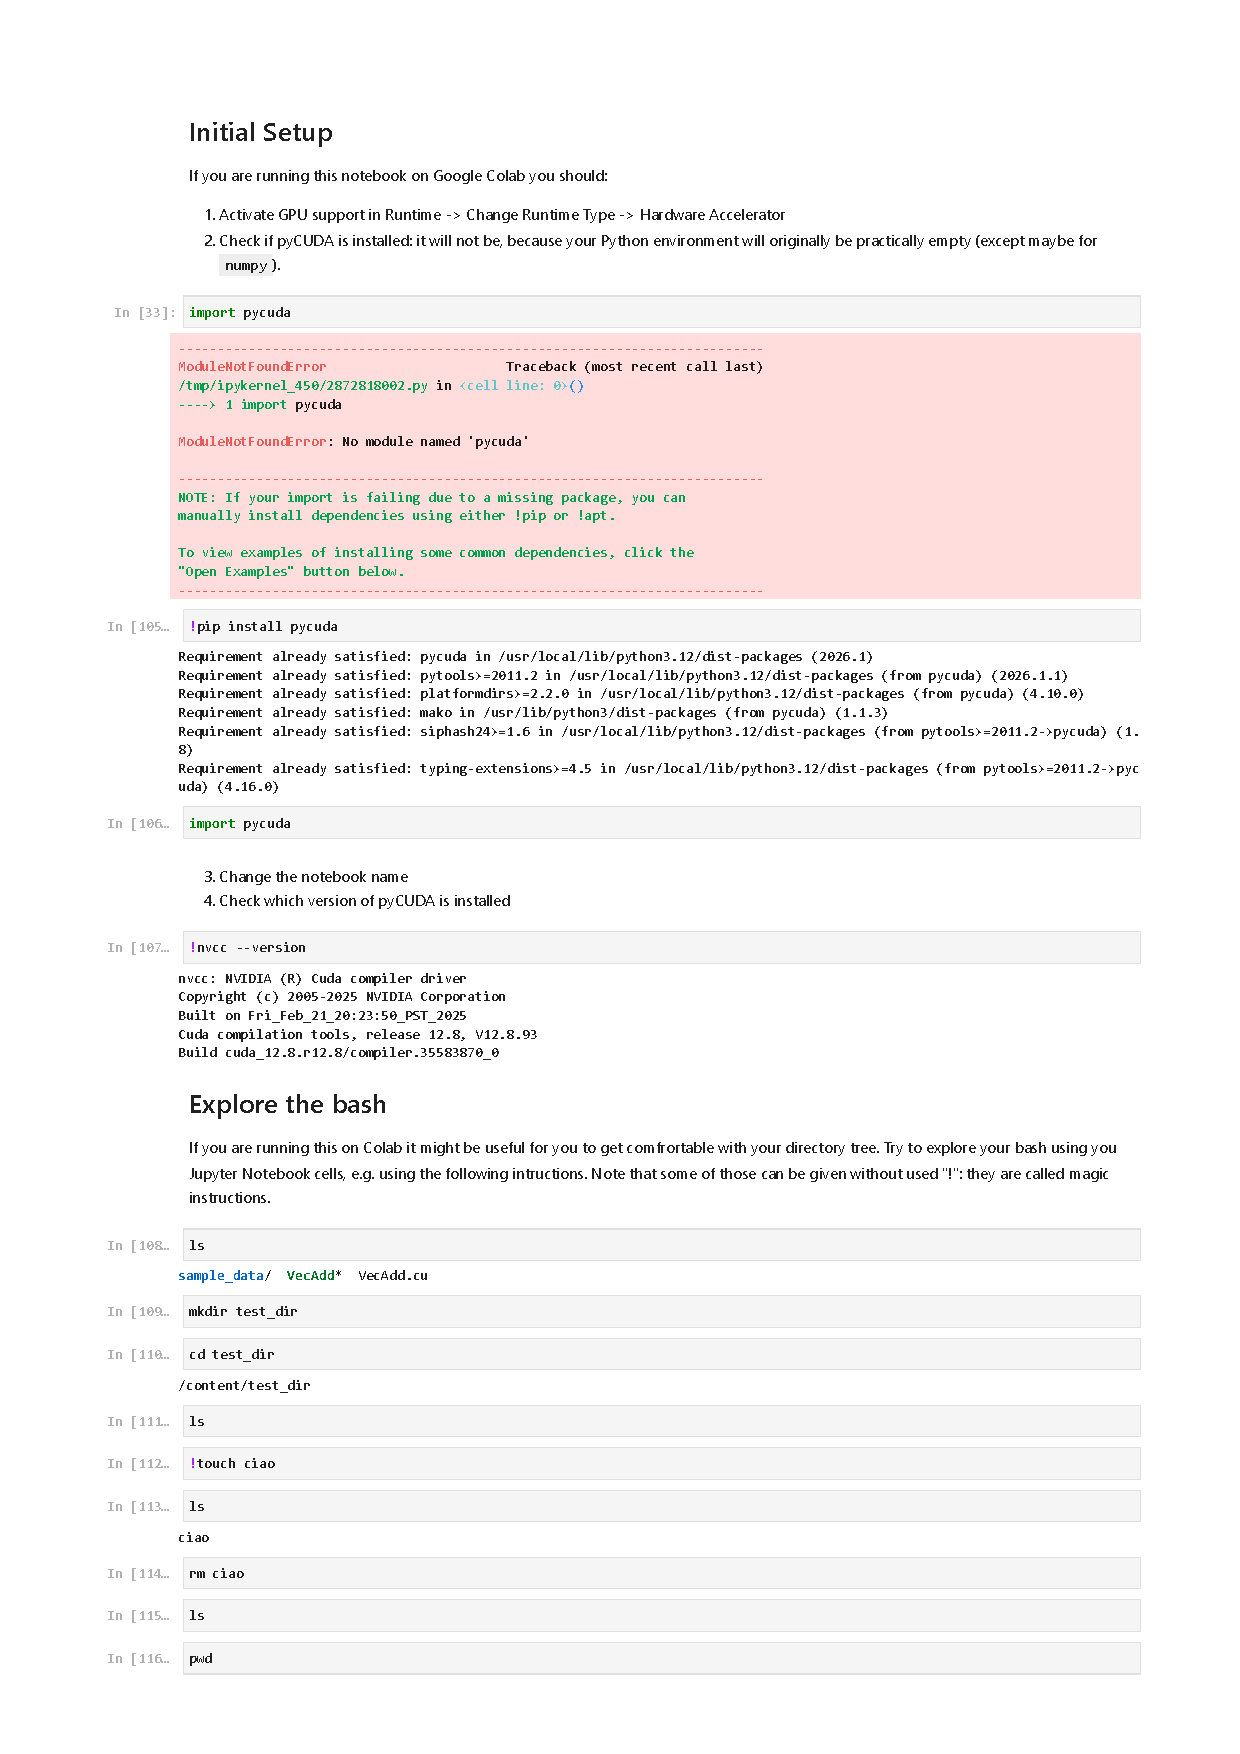
\includepdf[pages=-, pagecommand={\thispagestyle{plain}}]{lezioni/c_parallel5A_GPU.pdf}

\subsection{Bibliography}
\textbf{Parallel programming:}
\begin{itemize}
    \item[-] "The source book of parallel computing" (Dongarra et al.) - Morgan Kaufmann ed. (2003)
    \item[-] "Introduction to parallel programming" (Grama-Gupta-Karypis-Kumar)
\end{itemize}
\textbf{Parallel processing in Python:}
\begin{itemize}
    \item[-] \url{https://docs.python.org/2/library/multiprocessing.html}
    \item[-] \url{https://docs.python.org/3/library/threading.html}
\end{itemize}
\textbf{GPU online resources:}
\begin{itemize}
    \item[-] \url{https://docs.nvidia.com/cuda/index.html}
    \item[-] \url{https://docs.nvidia.com/pdf/CUDA_C_Programming_Guide.pdf}
    \item[-] \url{https://docs.nvidia.com/pdf/CUDA_C_Best_Practices_Guide.pdf}
    \item[-] \url{https://hgpu.org/} (collection of tutorials and articles)
\end{itemize}
\textbf{GPU books:}
\begin{itemize}
    \item[-] "GPU Computing and Applications" (Yiju Cai) - Springer
    \item[-] "Multicore and GPU programming: an integrated approach" (Barlas) - Morgan Kaufmann
    \item[-] "Cuda by Example" (Sanders) - Addison-Wesley
    \item[-] "Professional Cuda C programming" (Cheng et al.) - Wrox
\end{itemize}
\textbf{GPU in Python:}
\begin{itemize}
    \item[-] \url{https://wish4book.com/education/5410-hands-on-gpu-computing-with-python.html}
    \item[-] \url{https://documen.tician.de/pycuda/}
\end{itemize}